\documentclass[preprint,12pt,authoryear]{elsarticle}

\usepackage[T1]{fontenc}
\usepackage{lmodern}
\usepackage{amsmath,amssymb,amsthm}
\usepackage{booktabs}
\usepackage{graphicx}
\usepackage{xcolor}
\usepackage{algorithm}
\usepackage[noend]{algpseudocode}
\usepackage{tikz}
\usetikzlibrary{positioning,calc,arrows.meta,fit}
\usepackage{placeins}
\usepackage{url}
\usepackage[hidelinks]{hyperref}
\usepackage[margin=2.5cm]{geometry}

\setlength{\emergencystretch}{2em}
\newtheorem{proposition}{Proposition}
\newtheorem{corollary}{Corollary}
\theoremstyle{remark}
\newtheorem{remark}{Remark}
\algrenewcommand\algorithmicrequire{\textbf{Input:}}
\algrenewcommand\algorithmicensure{\textbf{Output:}}
\newcommand{\pending}[1]{\textcolor{red}{[PENDING: #1]}}

% generated by scripts/eswa_paper_assets.py -- do not edit
\providecommand\res[1]{\csname res@#1\endcsname}
\expandafter\def\csname res@H1-meanA\endcsname{0.590}
\expandafter\def\csname res@H1-medA\endcsname{0.500}
\expandafter\def\csname res@H1-neq\endcsname{6}
\expandafter\def\csname res@H1-ngt\endcsname{14}
\expandafter\def\csname res@H1-nlt\endcsname{8}
\expandafter\def\csname res@H1-p\endcsname{0.031}
\expandafter\def\csname res@H1-pholm\endcsname{0.043}
\expandafter\def\csname res@H1-pholm-pratt\endcsname{0.056}
\expandafter\def\csname res@H1-pholm-zsplit\endcsname{0.057}
\expandafter\def\csname res@H1-sigagainst\endcsname{1}
\expandafter\def\csname res@H1-sigfor\endcsname{5}
\expandafter\def\csname res@H2-meanA\endcsname{0.593}
\expandafter\def\csname res@H2-medA\endcsname{0.514}
\expandafter\def\csname res@H2-neq\endcsname{5}
\expandafter\def\csname res@H2-ngt\endcsname{15}
\expandafter\def\csname res@H2-nlt\endcsname{8}
\expandafter\def\csname res@H2-p\endcsname{0.022}
\expandafter\def\csname res@H2-pholm\endcsname{0.043}
\expandafter\def\csname res@H2-pholm-pratt\endcsname{0.056}
\expandafter\def\csname res@H2-pholm-zsplit\endcsname{0.057}
\expandafter\def\csname res@H2-sigagainst\endcsname{0}
\expandafter\def\csname res@H2-sigfor\endcsname{6}
\expandafter\def\csname res@S1-H1-B20-medA\endcsname{0.519}
\expandafter\def\csname res@S1-H1-C10-medA\endcsname{0.500}
\expandafter\def\csname res@S1-H1-C20-medA\endcsname{0.559}
\expandafter\def\csname res@S1-H1-FIR-medA\endcsname{0.613}
\expandafter\def\csname res@S1-H1-medA\endcsname{0.520}
\expandafter\def\csname res@S1-H1-p\endcsname{\ensuremath{7.7{\times}10^{-4}}}
\expandafter\def\csname res@S1-H1-sigagainst\endcsname{1}
\expandafter\def\csname res@S1-H1-sigfor\endcsname{12}
\expandafter\def\csname res@S1-H2-B20-medA\endcsname{0.504}
\expandafter\def\csname res@S1-H2-C10-medA\endcsname{0.522}
\expandafter\def\csname res@S1-H2-C20-medA\endcsname{0.611}
\expandafter\def\csname res@S1-H2-FIR-medA\endcsname{0.703}
\expandafter\def\csname res@S1-H2-medA\endcsname{0.529}
\expandafter\def\csname res@S1-H2-p\endcsname{\ensuremath{5.2{\times}10^{-4}}}
\expandafter\def\csname res@S1-H2-sigagainst\endcsname{0}
\expandafter\def\csname res@S1-H2-sigfor\endcsname{14}
\expandafter\def\csname res@abl-BBOB-D20-runs\endcsname{10}
\expandafter\def\csname res@abl-CEC2022-runs\endcsname{10}
\expandafter\def\csname res@abl-FIR-runs\endcsname{10}
\expandafter\def\csname res@acc-B20-10-EIG50\endcsname{4.4}
\expandafter\def\csname res@acc-B20-10-MPHBS\endcsname{0.6}
\expandafter\def\csname res@acc-B20-10-RND\endcsname{0.4}
\expandafter\def\csname res@acc-B20-11-EIG50\endcsname{1.0}
\expandafter\def\csname res@acc-B20-11-MPHBS\endcsname{0.0}
\expandafter\def\csname res@acc-B20-11-RND\endcsname{0.0}
\expandafter\def\csname res@acc-B20-14-EIG50\endcsname{2.8}
\expandafter\def\csname res@acc-B20-14-MPHBS\endcsname{2.7}
\expandafter\def\csname res@acc-B20-14-RND\endcsname{3.6}
\expandafter\def\csname res@acc-B20-2-EIG50\endcsname{1.5}
\expandafter\def\csname res@acc-B20-2-MPHBS\endcsname{1.9}
\expandafter\def\csname res@acc-B20-2-RND\endcsname{3.3}
\expandafter\def\csname res@box-list\endcsname{C10 F7, C10 F2, C20 F1, C20 F9, B20 f19, B20 f11, FIR Case 3, FIR Case 1}
\expandafter\def\csname res@common-loss\endcsname{13}
\expandafter\def\csname res@common-n\endcsname{336}
\expandafter\def\csname res@common-win\endcsname{260}
\expandafter\def\csname res@conv-C20\endcsname{1}
\expandafter\def\csname res@conv-FIR\endcsname{3}
\expandafter\def\csname res@ea4eig-D10-better\endcsname{0}
\expandafter\def\csname res@ea4eig-D10-tie\endcsname{4}
\expandafter\def\csname res@ea4eig-D10-worse\endcsname{8}
\expandafter\def\csname res@ea4eig-D20-better\endcsname{0}
\expandafter\def\csname res@ea4eig-D20-tie\endcsname{2}
\expandafter\def\csname res@ea4eig-D20-worse\endcsname{10}
\expandafter\def\csname res@f10-CMA-ES\endcsname{0}
\expandafter\def\csname res@f10-EIG50\endcsname{8.47}
\expandafter\def\csname res@f10-L-SHADE\endcsname{0}
\expandafter\def\csname res@f10-MPHBS\endcsname{121}
\expandafter\def\csname res@f10-RND\endcsname{89.9}
\expandafter\def\csname res@f10-ratio-MPHBS\endcsname{14.3}
\expandafter\def\csname res@f10-ratio-RND\endcsname{10.6}
\expandafter\def\csname res@f15-CMA-ES\endcsname{2.98}
\expandafter\def\csname res@f15-EIG50\endcsname{54.2}
\expandafter\def\csname res@f15-L-SHADE\endcsname{4.13}
\expandafter\def\csname res@f15-MPHBS\endcsname{51.2}
\expandafter\def\csname res@f15-RND\endcsname{58.7}
\expandafter\def\csname res@f3-CMA-ES\endcsname{8.95}
\expandafter\def\csname res@f3-EIG50\endcsname{1.99}
\expandafter\def\csname res@f3-L-SHADE\endcsname{0}
\expandafter\def\csname res@f3-MPHBS\endcsname{0.995}
\expandafter\def\csname res@f3-RND\endcsname{0.995}
\expandafter\def\csname res@friedman-B20\endcsname{\ensuremath{2.8{\times}10^{-26}}}
\expandafter\def\csname res@friedman-C10\endcsname{\ensuremath{3.9{\times}10^{-14}}}
\expandafter\def\csname res@friedman-C20\endcsname{\ensuremath{1.3{\times}10^{-14}}}
\expandafter\def\csname res@friedman-FIR\endcsname{\ensuremath{1.4{\times}10^{-12}}}
\expandafter\def\csname res@loss-CMA-ES\endcsname{31}
\expandafter\def\csname res@loss-DE\endcsname{6}
\expandafter\def\csname res@loss-GWO\endcsname{0}
\expandafter\def\csname res@loss-HBA\endcsname{0}
\expandafter\def\csname res@loss-L-SHADE\endcsname{34}
\expandafter\def\csname res@loss-MPA\endcsname{6}
\expandafter\def\csname res@loss-MPHBS\endcsname{0}
\expandafter\def\csname res@loss-PSO\endcsname{1}
\expandafter\def\csname res@loss-RND\endcsname{1}
\expandafter\def\csname res@loss-WOA\endcsname{0}
\expandafter\def\csname res@overhead-max\endcsname{5.5}
\expandafter\def\csname res@overhead-min\endcsname{3.2}
\expandafter\def\csname res@pos-CMA-ES\endcsname{2}
\expandafter\def\csname res@pos-DE\endcsname{7}
\expandafter\def\csname res@pos-EIG50\endcsname{3}
\expandafter\def\csname res@pos-EIG50-B20\endcsname{3}
\expandafter\def\csname res@pos-EIG50-C10\endcsname{1}
\expandafter\def\csname res@pos-EIG50-C20\endcsname{3}
\expandafter\def\csname res@pos-EIG50-FIR\endcsname{3}
\expandafter\def\csname res@pos-GWO\endcsname{10}
\expandafter\def\csname res@pos-HBA\endcsname{8}
\expandafter\def\csname res@pos-L-SHADE\endcsname{1}
\expandafter\def\csname res@pos-MPA\endcsname{6}
\expandafter\def\csname res@pos-MPHBS\endcsname{5}
\expandafter\def\csname res@pos-PSO\endcsname{9}
\expandafter\def\csname res@pos-RND\endcsname{4}
\expandafter\def\csname res@pos-WOA\endcsname{11}
\expandafter\def\csname res@rank-CMA-ES\endcsname{2.97}
\expandafter\def\csname res@rank-DE\endcsname{6.38}
\expandafter\def\csname res@rank-EIG50\endcsname{4.01}
\expandafter\def\csname res@rank-GWO\endcsname{9.27}
\expandafter\def\csname res@rank-HBA\endcsname{7.67}
\expandafter\def\csname res@rank-L-SHADE\endcsname{2.60}
\expandafter\def\csname res@rank-MPA\endcsname{4.88}
\expandafter\def\csname res@rank-MPHBS\endcsname{4.64}
\expandafter\def\csname res@rank-PSO\endcsname{8.22}
\expandafter\def\csname res@rank-RND\endcsname{4.62}
\expandafter\def\csname res@rank-WOA\endcsname{10.73}
\expandafter\def\csname res@runs-arms\endcsname{11}
\expandafter\def\csname res@runs-total\endcsname{18{,}840}
\expandafter\def\csname res@win-CMA-ES\endcsname{8}
\expandafter\def\csname res@win-DE\endcsname{37}
\expandafter\def\csname res@win-GWO\endcsname{52}
\expandafter\def\csname res@win-HBA\endcsname{47}
\expandafter\def\csname res@win-L-SHADE\endcsname{4}
\expandafter\def\csname res@win-MPA\endcsname{24}
\expandafter\def\csname res@win-MPHBS\endcsname{14}
\expandafter\def\csname res@win-PSO\endcsname{44}
\expandafter\def\csname res@win-RND\endcsname{12}
\expandafter\def\csname res@win-WOA\endcsname{56}
\expandafter\def\csname res@wtl-CMA-ES\endcsname{8/17/31}
\expandafter\def\csname res@wtl-DE\endcsname{37/13/6}
\expandafter\def\csname res@wtl-GWO\endcsname{52/4/0}
\expandafter\def\csname res@wtl-HBA\endcsname{47/9/0}
\expandafter\def\csname res@wtl-L-SHADE\endcsname{4/18/34}
\expandafter\def\csname res@wtl-MPA\endcsname{24/26/6}
\expandafter\def\csname res@wtl-MPHBS\endcsname{14/42/0}
\expandafter\def\csname res@wtl-PSO\endcsname{44/11/1}
\expandafter\def\csname res@wtl-RND\endcsname{12/43/1}
\expandafter\def\csname res@wtl-WOA\endcsname{56/0/0}


\journal{Expert Systems with Applications}

\begin{document}

\begin{frontmatter}

\title{EIG-MPHBS: a rotation-invariant information exchange for hybrid Honey Badger--Marine Predators optimisation}

\author[1]{Abinaya G\corref{cor1}}
\ead{gabinaya@saveetha.ac.in}
\cortext[cor1]{Corresponding author.}
\affiliation[1]{organization={Department of Information Technology, Saveetha Engineering College},
                city={Chennai}, country={India}}

\begin{abstract}
Hybrid metaheuristics that run two populations side by side often share information by recombining their members
coordinate by coordinate. This exchange depends on the coordinate system: when the variables of a problem are coupled
by a rotation, recombining along the original axes breaks the structure that each population has found. We study this
weakness in MPHBS, a recent hybrid of the Honey Badger Algorithm and the Marine Predators Algorithm, and propose
EIG-MPHBS, which performs the exchange in the eigenvector frame of the covariance of both populations in half of the
iterations. The exchange step becomes provably invariant to rotations of the search space, uses exactly the same number
of function evaluations as the original and adds \res{overhead-min}--\res{overhead-max}\% to the run time. We evaluate
EIG-MPHBS in \res{runs-total} runs on CEC2022 ($D=10, 20$), the 24 BBOB functions ($D=20$) and eight FIR filter-design
problems, against MPHBS, its parent algorithms, four classical metaheuristics, L-SHADE and CMA-ES. In a test fixed
before the experiments on 28 held-out instances, EIG-MPHBS improves on both MPHBS and its budget-matched random-mediator
variant (Holm-adjusted $p=\res{H1-pholm}$); the margin is small and depends on how ties are treated. On all 56
instances it is never significantly worse than MPHBS, reduces the median error on the rotated ellipsoid
\res{f10-ratio-MPHBS}-fold, and beats HBA, MPA, PSO, DE, GWO and WOA on \res{common-win} of \res{common-n}
comparisons. It ranks third of eleven overall, behind L-SHADE and CMA-ES, and remains behind the CEC2022 entry EA4eig.
\end{abstract}

\begin{keyword}
Hybrid metaheuristics \sep Rotation invariance \sep Eigenvector crossover \sep Honey Badger Algorithm \sep
Marine Predators Algorithm \sep FIR filter design
\end{keyword}

\end{frontmatter}

%% =====================================================================
\section{Introduction}
\label{sec:intro}

Population-based metaheuristics are a standard tool for expert and intelligent systems that must optimise black-box
objectives, from controller and filter design to scheduling and model tuning. A popular way to improve them is
hybridisation: two algorithms with complementary search behaviour run together and exchange
information~\citep{talbi2002taxonomy,blum2011hybrid,ma2019multipop}. MPHBS~\citep{flores2026mphbs} is a recent example. It runs
a Honey Badger Algorithm (HBA) population~\citep{hashim2022hba} and a Marine Predators Algorithm (MPA)
population~\citep{faramarzi2020mpa} in parallel, and in every iteration a mediator assembles new candidate solutions
dimension by dimension from the best members of both populations. MPHBS was proposed with a SARSA-style learner that
chooses which population and which rank supplies each coordinate. A companion study~\citep{g2026deconstruction}
showed that a random choice at the same evaluation budget performs as well as the learner, and that the gains of MPHBS
come from the exchange step itself.

This exchange has a structural weakness that it shares with many recombination operators: it acts on the coordinates of
the search space. Copying coordinate $d$ from one solution into another is meaningful when the variables are separable,
but when the objective couples variables through a rotation, coordinate-wise recombination destroys the correlated
structure that the populations have learned~\citep{salomon1996rotation}. In MPHBS this shows up clearly on rotated
problems: on the BBOB rotated ellipsoid (f10), MPHBS ends with a median error of \res{f10-MPHBS}, while on its separable
counterpart (f2) it reaches the $10^{-8}$ accuracy floor (Section~\ref{sec:rotation}).

Eigenvector-based recombination is a known remedy. \citet{guo2015eigen} recombine differential evolution (DE) vectors in
the eigenvector frame of the population covariance, CoBiDE~\citep{wang2014cobide} does the same with covariance matrix
learning, EA4eig~\citep{bujok2022ea4eig} applies eigen crossover inside a cooperative model of four algorithms, and in
evolutionary multitasking \citet{tang2021regularized,tang2022adaptive} transfer knowledge between populations in
aligned eigen-subspaces. We do not propose a new operator. Our contribution is to identify the coordinate dependence of
the HBA--MPA mediator as a cause of its weakness on rotated problems, to give the hybrid a rotation-invariant exchange
that costs no extra evaluations, and to test the result rigorously against a broad set of algorithms. Specifically:

\begin{enumerate}
\item We propose EIG-MPHBS, which carries out the MPHBS exchange in the eigenvector frame of the pooled covariance of
both populations in half of the iterations and along the original axes in the other half
(Section~\ref{sec:method}).
\item We prove that the eigen-frame exchange is invariant to rotations of the search space and that it uses exactly the
same number of function evaluations as the axis-frame exchange, at an extra arithmetic cost of
$O(ND^2+D^3)$ per iteration (Section~\ref{sec:theory}).
\item We evaluate EIG-MPHBS on 56 instances from CEC2022, BBOB and an FIR filter-design application against ten
algorithms: MPHBS and its random-mediator variant, the parent algorithms HBA and MPA, four widely used metaheuristics
(PSO, DE, GWO, WOA), and two state-of-the-art references, L-SHADE and CMA-ES. We also compare with the official CEC2022
results of EA4eig (Section~\ref{sec:results}).
\item The main hypotheses, the held-out instances and the statistical tests were fixed in a design document before any
confirmatory run. Code, raw results and the scripts that produce every number in this paper are public.
\end{enumerate}

The results are positive but bounded, and we report both sides. EIG-MPHBS improves on MPHBS, is never significantly
worse than it on any of the 56 instances, and clearly outperforms the common metaheuristics, including both of its
parent algorithms. L-SHADE, CMA-ES and EA4eig remain stronger on most instances, and the confirmatory advantage on the
held-out instances, while significant under the test we fixed in advance, is small.

The paper is organised as follows. Section~\ref{sec:related} reviews related work, Section~\ref{sec:mphbs} describes
MPHBS, Section~\ref{sec:method} presents EIG-MPHBS and Section~\ref{sec:theory} its properties.
Section~\ref{sec:setup} describes the experimental setup, Section~\ref{sec:results} the results and
Section~\ref{sec:discussion} discusses them. Section~\ref{sec:conclusion} concludes.

%% =====================================================================
\section{Related work}
\label{sec:related}

\subsection{HBA, MPA and their hybrids}
HBA~\citep{hashim2022hba} alternates a digging move, scaled by a smell intensity, with a move towards the best agent,
both modulated by a decreasing density factor. MPA~\citep{faramarzi2020mpa} switches between Brownian and L\'evy
movements in three phases and adds a marine memory and a fish-aggregating-device (FAD) perturbation. Both have many
variants, hybrids and applications~\citep{hassan2024hba,albetar2023mpa}. HBA and MPA have been combined in series,
population-division and switching schemes for power-network planning~\citep{aldhaifallah2024mpahba}; MPHBS couples them
through a learned dimension-wise exchange~\citep{flores2026mphbs}, which \citet{g2026deconstruction} showed to be no
better than a budget-matched random choice.

\subsection{Rotation invariance and coordinate-wise recombination}
\citet{salomon1996rotation} showed that genetic algorithms with coordinate-wise operators lose much of their
performance when a separable function is rotated, because their success relies on the independence of the variables.
The same holds for binomial crossover in DE and for any operator that mixes solutions coordinate by coordinate. CMA-ES
avoids the problem by adapting a full covariance matrix and is invariant to rotations of the search
space~\citep{hansen2001cma}; this is one reason why benchmark suites such as BBOB~\citep{hansen2009bbob,hansen2021coco}
and CEC2022~\citep{kumar2021cec2022} include rotated functions.

\subsection{Eigenvector-based recombination}
Several operators recombine solutions in a coordinate system that follows the population. \citet{guo2015eigen} perform
DE crossover in the eigenvector frame of the population covariance with a given probability, and CoBiDE uses covariance
matrix learning in the same way~\citep{wang2014cobide}. \citet{civicioglu2018aplus} propose a rotation-invariant
crossover based on QR decomposition. EA4eig~\citep{bujok2022ea4eig}, a cooperative model of CMA-ES, CoBiDE, jSO and IDE
with eigen crossover, was among the strongest entries of the CEC2022 competition. In evolutionary multitasking,
\citet{tang2021regularized} project the individuals of two populations onto aligned eigen-subspaces before recombining
them, and \citet{tang2022adaptive} transfer knowledge between tasks in a coordinate system built from the major
eigenvectors of both populations. QLRUN~\citep{adam2027qlrun} combines Q-learning with covariance matrix learning in a
single metaheuristic.

\subsection{Positioning}
The idea of exchanging information between populations in an eigen frame of their joint distribution is therefore known;
the closest precedents are the inter-task transfers of \citet{tang2021regularized,tang2022adaptive}. A Scopus search
(title, abstract and keywords, 28~October~2026; queries in the repository) found no study that applies it to the
dimension-wise exchange of HBA--MPA hybrids or that analyses the rotation dependence of such mediators. Our contribution
is thus an application of a known principle to a new and recently popular class of hybrids, with a proof of its
invariance in this setting, a demonstration of its cost, and a comparison against a wide set of algorithms under a
design fixed in advance.

%% =====================================================================
\section{MPHBS}
\label{sec:mphbs}

We minimise $f:\Omega\to\mathbb{R}$ over a box $\Omega=[\ell,u]^D$; points are row vectors. MPHBS maintains an HBA
population $X^H\in\mathbb{R}^{N\times D}$ and an MPA population $X^M\in\mathbb{R}^{N\times D}$ ($N=30$ each), their best
members $p^H,p^M$, and the global best $p^\star$ with value $f^\star$. Each iteration has three stages
(Algorithm~\ref{alg:iteration}).

\paragraph{Phase 1: native moves} HBA and MPA each update their population with their own operators; each candidate is
evaluated and replaces its parent if better, and MPA applies its marine-memory rule. A FAD perturbation of the MPA
population follows, before Phase 2 on CEC2022 and BBOB and after it on FIR, as in the authors' configurations. Phase 1
costs $2N$ evaluations, the FAD stage $N$. A full description of the operators is given
by~\citet{flores2026mphbs} and~\citet{g2026deconstruction}.

\paragraph{Phase 2: the mediator} From each population the mediator takes a subset of
$N_\mathrm{sub}=\min(N,\max(5,\mathrm{round}(\rho N)))$ members (half of them the best, the rest at random), sorted by
fitness, and stacks them into a tensor $R\in\mathbb{R}^{N_\mathrm{sub}\times D\times 2}$, where $R_{n,d,c}$ is
coordinate $d$ of the rank-$n$ member of source $c\in\{H,M\}$. Starting from $v=p^\star$ (one evaluation), it runs
$E=N_\mathrm{sub}N_i$ episodes. The dimensions are split into five blocks of size $\lceil D/5\rceil$ visited along random
permutations. In episode $e$ with active block $A_e$, $K$ candidates are built: candidate $k$ copies $v$ and, for each
$d\in A_e$, sets $v'_d=R_{n_d,d,c_d}$ for a chosen source $c_d$ and rank $n_d$. In MPHBS the choice is made by policies
over a SARSA value table; in the random-mediator variant MPHBS-R it is drawn uniformly. A proxy score that needs no
evaluation,
\begin{equation}
s(v') = -w_\mathrm{rank}\,\overline{(n_d+1)}_{d\in A_e} + w_\mathrm{nov}\,\overline{|v'_d-v_d|}_{d\in A_e}
        - w_\mathrm{best}\,\|v'_{A_e}-p^\star_{A_e}\|_2,
\label{eq:proxy}
\end{equation}
selects one candidate, which is evaluated (one evaluation per episode). It is accepted if it improves $f(v)$, and
otherwise with a small probability that decreases over the run. Accepted candidates replace the worst subset members
that they improve, and a new global best is copied into both subsets. At the end of Phase 2 the subsets are written back.

\paragraph{Configurations} We use the authors' configurations: $K=7$, $N_i=3$, $\rho=0.25$ (so $N_\mathrm{sub}=8$,
$E=24$) on CEC2022 and BBOB, and $K=3$, $N_i=9$ ($E=72$) on FIR, with $w_\mathrm{rank}=1$, $w_\mathrm{nov}=0.3$,
$w_\mathrm{best}=0.05$. One iteration costs $3N+1+E$ evaluations.

%% =====================================================================
\section{EIG-MPHBS}
\label{sec:method}

\subsection{Why the exchange depends on the coordinate system}
The mediator builds each candidate by taking coordinate $d$ from one stored solution and coordinate $d'$ from another.
If the objective is separable, this is a sound way to combine good partial solutions. If the objective is
$f(x)=g(xQ)$ for a rotation $Q$, the meaningful directions are the columns of $Q$, and a candidate assembled from the
coordinates of different solutions generally lies far from all of them along those directions. Its value is then poor
even when every source solution is good, so few exchange candidates are accepted and the exchange contributes little.
The populations themselves carry the information needed to correct this: on such problems their spread aligns with the
shape of the basin they occupy, so the principal axes of their covariance approximate the directions of the problem.

\subsection{The eigen-frame exchange}
At the start of Phase 2, with probability $q$, EIG-MPHBS computes the sample covariance of the pooled populations,
\begin{equation}
C = \mathrm{cov}\!\begin{pmatrix} X^H \\ X^M \end{pmatrix} = B\Lambda B^\top,
\label{eq:cov}
\end{equation}
with an orthonormal eigenvector matrix $B$ (columns ordered by eigenvalue). All mediator operations of the iteration are
then performed on the coordinates $z=xB$ instead of $x$: the tensor $R$ holds the projected subsets, the start point is
$z=p^\star B$, candidates are assembled coordinate-wise in $z$, and the proxy score~\eqref{eq:proxy} is computed in $z$.
The selected candidate is mapped back and clipped to the box, $x'=\mathrm{clip}(z'B^\top)$, and evaluated; if it is
accepted, its eigen coordinates are recomputed from the clipped point, $z\leftarrow x'B$. With probability $1-q$ the
iteration uses the original axes ($B=I$), so the method reduces to MPHBS-R in those iterations.

EIG-MPHBS uses the random mediator of MPHBS-R, not the SARSA learner, because the learner brings no benefit at the same
budget~\citep{g2026deconstruction} and its value table is indexed by coordinates, whose meaning would change whenever
the frame changes. We set $q=0.5$. This keeps the axis frame available for separable or nearly separable structure, on
which coordinate-wise exchange is effective, while using the eigen frame for coupled structure. The value $q=0.5$ was
chosen over $q=1$ in a 10-run pilot on 32 instances (BBOB f1, f3, f8, f10, f12, f15, f16, f21; CEC2022 $D=20$; FIR);
those instances are excluded from the confirmatory test (Section~\ref{sec:design}). Algorithm~\ref{alg:iteration}
summarises one iteration and Fig.~\ref{fig:scheme} the exchange.

\begin{algorithm}[t]
\caption{One iteration of EIG-MPHBS. Lines~\ref{line:frame}--\ref{line:back} are the only differences from MPHBS-R.}
\label{alg:iteration}
\small
\begin{algorithmic}[1]
\Require populations $X^H,X^M$, global best $p^\star$, iteration $t$, eigen-frame probability $q$
\State HBA and MPA moves; evaluate; greedy replacement; marine memory \Comment{$2N$ FEs}
\If{FAD before Phase 2} FAD stage \Comment{$N$}\EndIf
\State $p^\star\gets$ best of $p^H,p^M$
\State \textbf{if} $U(0,1)<q$ \textbf{then} $B\gets$ eigenvectors of $\mathrm{cov}([X^H;X^M])$ \textbf{else} $B\gets I$
\Comment{0 FEs} \label{line:frame}
\State draw ranked subsets $S^H,S^M$; $R\gets$ projected subsets $S^HB$, $S^MB$; $z\gets p^\star B$; $f_z\gets f(p^\star)$
\Comment{1}
\For{$e=1,\dots,E$}
  \State $A_e\gets$ next block of dimensions
  \State for $k=1..K$: $z^{(k)}\gets z$; for $d\in A_e$ draw $(c_d,n_d)$ uniformly; $z^{(k)}_d\gets R_{n_d,d,c_d}$
  \State $z'\gets\arg\max_k s(z^{(k)})$ \eqref{eq:proxy}; $x'\gets\mathrm{clip}(z'B^\top)$; $f'\gets f(x')$
  \Comment{1} \label{line:back}
  \If{accepted} $z\gets x'B$, $f_z\gets f'$; update $S^H,S^M$ and their projections in $R$\EndIf
  \If{$f'<f^\star$} $p^\star\gets x'$; copy $x'$ into a random row of $S^H$ and $S^M$\EndIf
\EndFor
\State write $S^H,S^M$ back into $X^H,X^M$; update $p^H,p^M,p^\star$
\If{FAD after Phase 2} FAD stage \Comment{$N$}\EndIf
\end{algorithmic}
\end{algorithm}

\begin{figure}[t]
\centering
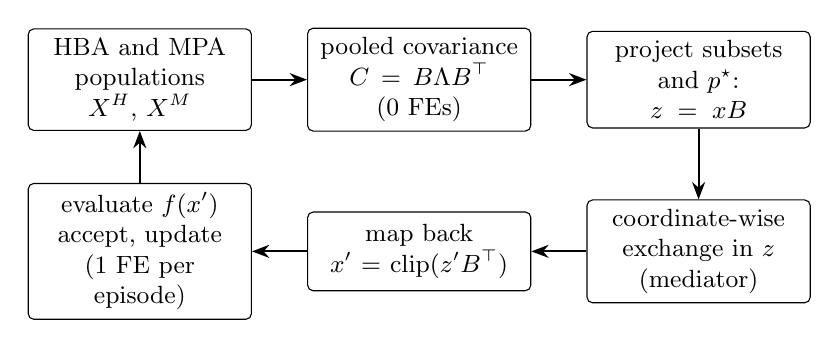
\begin{tikzpicture}[
  box/.style={draw, rounded corners=2pt, align=center, font=\small, minimum height=1.0cm, text width=2.6cm},
  arr/.style={-{Stealth[length=2.2mm]}, thick}]
\node[box] (pop) {HBA and MPA\\populations\\$X^H$, $X^M$};
\node[box, right=0.7cm of pop] (cov) {pooled covariance\\$C=B\Lambda B^\top$\\(0 FEs)};
\node[box, right=0.7cm of cov] (proj) {project subsets\\and $p^\star$:\\$z = xB$};
\node[box, below=0.9cm of proj] (rec) {coordinate-wise\\exchange in $z$\\(mediator)};
\node[box, left=0.7cm of rec] (back) {map back\\$x'=\mathrm{clip}(z'B^\top)$};
\node[box, left=0.7cm of back] (eval) {evaluate $f(x')$\\accept, update\\(1 FE per episode)};
\draw[arr] (pop) -- (cov);
\draw[arr] (cov) -- (proj);
\draw[arr] (proj) -- (rec);
\draw[arr] (rec) -- (back);
\draw[arr] (back) -- (eval);
\draw[arr] (eval) -- (pop);
\end{tikzpicture}
\caption{The eigen-frame exchange of EIG-MPHBS in one iteration (used with probability $q=0.5$; otherwise $B=I$).}
\label{fig:scheme}
\end{figure}

%% =====================================================================
\section{Properties}
\label{sec:theory}

\begin{proposition}[Rotation invariance of the exchange]
\label{prop:invariance}
Let $Q$ be an orthogonal matrix and consider the rotated problem $\tilde f(y)=f(yQ^\top)$. Suppose the populations,
subsets and global best of the rotated run are the rotated images $\tilde X = XQ$ of those of the original run, the
pooled covariance has distinct eigenvalues, the same random numbers are drawn, and no clipping occurs. Then the
eigen-frame exchange produces, in every episode, the candidate $\tilde x'=x'Q$, with the same objective value and the
same acceptance decision.
\end{proposition}

\begin{proof}
The pooled covariance of the rotated populations is $\tilde C=Q^\top CQ$, which has the same eigenvalues as $C$ and,
since they are distinct, eigenvectors $\tilde B=Q^\top BS$ with $S$ a diagonal matrix of signs, in the same order. The
eigen coordinates of a rotated point are therefore $\tilde z = xQ\,Q^\top BS = zS$: each coordinate equals the original
one up to a fixed sign. Ranks depend only on objective values, which are equal because $\tilde f(xQ)=f(x)$. Assembling a
candidate by copying coordinate $d$ from a stored solution commutes with multiplication by $S$, so $\tilde z'=z'S$.
The terms of the proxy score~\eqref{eq:proxy} are a mean rank, a mean of absolute coordinate differences and a
Euclidean norm, all unchanged by sign flips, so the same candidate is selected. Mapping back gives
$\tilde x'=\tilde z'\tilde B^\top = z'SS^\top B^\top Q = x'Q$, whose value is $\tilde f(x'Q)=f(x')$, and the
acceptance rule depends only on objective values.
\end{proof}

\begin{remark}
The axis-frame exchange ($B=I$) has no such property: rotating the problem changes which coordinates are copied
together. Proposition~\ref{prop:invariance} concerns the exchange step only. The HBA and MPA moves of Phase 1 are
coordinate-wise and not rotation invariant, and neither is clipping to the box, so EIG-MPHBS as a whole is not
rotation invariant. A unit test in the repository checks the invariance of the eigen coordinates numerically.
\end{remark}

\begin{proposition}[No extra evaluations]
\label{prop:cost}
In every iteration EIG-MPHBS performs exactly the same number of function evaluations as MPHBS-R, $3N+1+E$. The
additional arithmetic cost is $O(ND^2+D^3)$ for the covariance and its eigendecomposition and $O(D^2)$ per episode for
the projections, i.e.\ $O(ND^2+D^3+ED^2)$ per iteration.
\end{proposition}

\begin{proof}
The frame is computed from points already evaluated, and the mediator evaluates one start point and one candidate per
episode in either frame. The covariance of $2N$ points costs $O(ND^2)$, the symmetric eigendecomposition $O(D^3)$, and
each projection or back-projection of a $D$-vector $O(D^2)$.
\end{proof}

For $D\le 31$ and $N=30$ this overhead is negligible compared with the cost of the objective evaluations and the
mediator itself; Section~\ref{sec:cost} measures it. A unit test checks that EIG-MPHBS and MPHBS-R use identical
evaluation counts on every run.

%% =====================================================================
\section{Experimental setup}
\label{sec:setup}

\subsection{Benchmarks}
We use four benchmark sets (56 instances):
\begin{itemize}
\item CEC2022~\citep{kumar2021cec2022}, F1--F12, at $D=10$ and $D=20$ (24 instances), computed with the official code.
\item BBOB~\citep{hansen2009bbob}, f1--f24 at $D=20$, with problem instance $((r-1)\bmod 15)+1$ in run $r$. The suite
contains separable and rotated versions of the same functions, which allows a direct test of rotation dependence.
\item Eight FIR filter-design problems from the MPHBS study~\citep{flores2026mphbs} ($D=31$): low-pass, high-pass,
band-pass and band-stop filters, each in an easier and a harder variant, with coefficients $h\in[-1,1]^{31}$ and the
objective
\begin{equation}
F(h) = W_p\,\frac{1}{|P|}\sum_{n\in P}\bigl(|H(\omega_n)|-1\bigr)^2 + W_s\,\frac{1}{|S|}\sum_{n\in S}|H(\omega_n)|^2,
\label{eq:fir}
\end{equation}
where $H$ is the 2048-point discrete Fourier transform of $h$, $P$ and $S$ are the pass- and stop-band grid points,
$W_p=1$ and $W_s\in\{100,120\}$.
\end{itemize}
The budget is $2\times10^5$ evaluations on CEC2022 and BBOB and $1.5\times10^5$ on FIR. Each algorithm is run 30 times
per instance. The outcome is the final error $f(x_\mathrm{best})-f^\star$ (the objective value on FIR), floored at
$10^{-8}$.

\subsection{Algorithms}
Table~\ref{tab:algos} lists the eleven algorithms. MPHBS, MPHBS-R and EIG-MPHBS share all code except the flags shown.
HBA and MPA are the parent algorithms as ported in our framework, which was validated against the MPHBS authors' MATLAB
results (no significant differences in 80 distribution comparisons on CEC2022 and FIR). PSO, DE, GWO and WOA are four
widely used metaheuristics with their published default settings, and L-SHADE~\citep{tanabe2014lshade} and
CMA-ES with IPOP restarts~\citep{hansen2001cma,auger2005ipop,hansen2019pycma} are state-of-the-art references. All
algorithms use the same budget; the classical ones stop exactly at the budget, while the MPHBS family stops after the
last complete iteration (199\,930 of 200\,000 evaluations on CEC2022 and BBOB, 149\,857 of 150\,000 on FIR). No
algorithm was tuned on our benchmarks beyond the choice of $q$ described above.

\begin{table*}[t]
\centering
\caption{Algorithms and settings. $N$: population size; HBA--MPA hybrids run two populations of $N$ each.}
\label{tab:algos}
\small
\begin{tabular}{p{2.4cm}p{12.6cm}}
\toprule
Algorithm & Settings \\
\midrule
EIG-MPHBS & proposed; MPHBS with random mediator and eigen-frame exchange with probability $q=0.5$; $N=30$ \\
MPHBS-R & MPHBS with a uniform random mediator at the same budget~\citep{g2026deconstruction}; $N=30$ \\
MPHBS & as published, SARSA mediator~\citep{flores2026mphbs}; $N=30$; $K,N_i,\rho$ as in Section~\ref{sec:mphbs} \\
HBA & \citet{hashim2022hba}; $N=30$, $\beta=6$, $C=2$ \\
MPA & \citet{faramarzi2020mpa}; $N=30$, $P=0.5$, FADs $=0.2$ \\
PSO & global best, inertia $0.9\to0.4$~\citep{kennedy1995pso,shi1998inertia}; $c_1=c_2=2$, $|v|\le0.2(u-\ell)$; $N=30$ \\
DE & DE/rand/1/bin~\citep{storn1997de}; $F=0.5$, $CR=0.9$; $N=30$ \\
GWO & \citet{mirjalili2014gwo}; $a: 2\to0$; $N=30$ \\
WOA & \citet{mirjalili2016woa}; $a: 2\to0$, $b=1$; $N=30$ \\
L-SHADE & \citet{tanabe2014lshade}; $N_\mathrm{init}=18D$, $N_\mathrm{min}=4$, $H=6$, archive rate 2.6, $p=0.11$ \\
CMA-ES & IPOP-CMA-ES~\citep{auger2005ipop}, pycma~\citep{hansen2019pycma}; $\sigma_0=0.3(u-\ell)$, default $\lambda$,
population doubled at each restart \\
\bottomrule
\end{tabular}
\end{table*}

\subsection{Design and statistics}
\label{sec:design}
Runs with the same benchmark, instance and run number share their seed across all algorithms, so comparisons are
paired. Before any confirmatory run we fixed in a design document the arms, the benchmarks and two hypotheses on a
held-out set of 28 instances that were not used in any pilot: CEC2022 $D=10$ F1--F12 and BBOB f2, f4--f7, f9, f11, f13,
f14, f17--f20, f22--f24. For each instance we compute the Vargha--Delaney effect size~\citep{vargha2000}
$A=P(e_1<e_2)+\tfrac12P(e_1=e_2)$ over all $30\times30$ pairs of final errors, where $e_1$ belongs to EIG-MPHBS.
\begin{itemize}
\item \textbf{H1}: EIG-MPHBS outperforms MPHBS-R, i.e.\ the median of $A$ over the held-out instances exceeds 0.5.
This isolates the effect of the eigen frame.
\item \textbf{H2}: EIG-MPHBS outperforms MPHBS.
\end{itemize}
Each is tested with a one-sided Wilcoxon signed-rank test~\citep{wilcoxon1945} of $A-0.5$ over the 28 instances, with
Holm correction~\citep{holm1979} over the two hypotheses at $\alpha=0.05$. All other analyses are secondary and
descriptive: the same statistics on all 56 instances; per-instance paired Wilcoxon tests with Holm correction within
each benchmark; Friedman ranks~\citep{derrac2011tutorial,demsar2006}; the rotation pairs of BBOB; the comparison with
EA4eig; and run time. The six classical algorithms were added after the main analysis to provide the comparisons that
are customary in this field; their addition is recorded in the design document and does not affect H1 and H2.

%% =====================================================================
\section{Results}
\label{sec:results}

\subsection{Confirmatory tests}
Table~\ref{tab:confirm} and Fig.~\ref{fig:heldout} show the confirmatory results. On the held-out instances, EIG-MPHBS
is better than MPHBS-R on \res{H1-ngt} instances, tied on \res{H1-neq} and worse on \res{H1-nlt} (one-sided
$p=\res{H1-p}$), and better than MPHBS on \res{H2-ngt}, tied on \res{H2-neq} and worse on \res{H2-nlt}
($p=\res{H2-p}$). After Holm correction both hypotheses are supported ($p_\text{Holm}=\res{H1-pholm}$ for each). The
evidence is not strong, however. The median effect is small (\res{H1-medA} and \res{H2-medA}), because most CEC2022
$D=10$ functions are solved equally well by all three variants, and when the instances with $A=0.5$ are kept in the
test with Pratt or zero-split handling the Holm-adjusted $p$-values become \res{H1-pholm-pratt} and
\res{H1-pholm-zsplit}. The decision rule fixed in advance used the default handling, which drops these instances; we
report the alternatives so that readers can weigh the result.

The per-instance tests show where the effect comes from. Against MPHBS-R, EIG-MPHBS is significantly better on
\res{H1-sigfor} held-out instances (BBOB f6, f9, f11, f14, f19) and worse on \res{H1-sigagainst} (f4, the separable
Rastrigin with asymmetric penalty). Against MPHBS it is better on \res{H2-sigfor} and never significantly worse. The
gains are concentrated on BBOB functions with ill-conditioned or rotated structure.

On all 56 instances, including the 28 used in the pilot or not held out, the picture is clearer: the median $A$ is
\res{S1-H1-medA} against MPHBS-R ($p=\res{S1-H1-p}$; \res{S1-H1-sigfor} instances significantly better, \res{S1-H1-sigagainst}
worse) and \res{S1-H2-medA} against MPHBS ($p=\res{S1-H2-p}$; \res{S1-H2-sigfor} better, \res{S1-H2-sigagainst}
worse). The largest effects are on FIR (median $A$ \res{S1-H2-FIR-medA} against MPHBS) and CEC2022 $D=20$
(\res{S1-H2-C20-medA}). These instances include the pilot instances on which $q$ was chosen, so their effect sizes may
be optimistic.

% generated by scripts/eswa_paper_assets.py -- do not edit
\begin{table*}[t]
\centering
\caption{Confirmatory tests on the 28 held-out instances (H1, H2) and their repetition on all 56 instances
(H1$'$, H2$'$, secondary: the 28 additional instances include those used to choose the eigen-frame probability).
$\tilde A$: median Vargha--Delaney effect over instances ($>0.5$ favours EIG-MPHBS). W/T/L: instances with
$A>0.5$, $A=0.5$, $A<0.5$. $p$: one-sided Wilcoxon signed-rank test of $A-0.5$ over instances; Holm over
\{H1, H2\}. The two sensitivity columns keep the instances with $A=0.5$ (Pratt and zero-split handling).
Sig.: instances where a paired per-instance test (Holm within benchmark) favours EIG-MPHBS / the comparator.}
\label{tab:confirm}
\footnotesize
\setlength{\tabcolsep}{4pt}
\resizebox{\textwidth}{!}{%
\begin{tabular}{llccccccc}
\toprule
 & Comparison & $\tilde A$ & W/T/L & $p$ & $p_\text{Holm}$ & $p_\text{Holm}$ (Pratt) & $p_\text{Holm}$ (zsplit) & Sig. \\
\midrule
H1 & EIG-MPHBS vs MPHBS-R & 0.500 & 14/6/8 & 0.031 & 0.043 & 0.056 & 0.057 & 5/1 \\
H2 & EIG-MPHBS vs MPHBS & 0.514 & 15/5/8 & 0.022 & 0.043 & 0.056 & 0.057 & 6/0 \\
\midrule
H1$'$ & all 56 instances (vs MPHBS-R) & 0.520 & 31/7/18 & \ensuremath{7.7{\times}10^{-4}} & -- & -- & -- & 12/1 \\
H2$'$ & all 56 instances (vs MPHBS) & 0.529 & 33/6/17 & \ensuremath{5.2{\times}10^{-4}} & -- & -- & -- & 14/0 \\
\bottomrule
\end{tabular}}
\end{table*}


\begin{figure}[t]
\centering
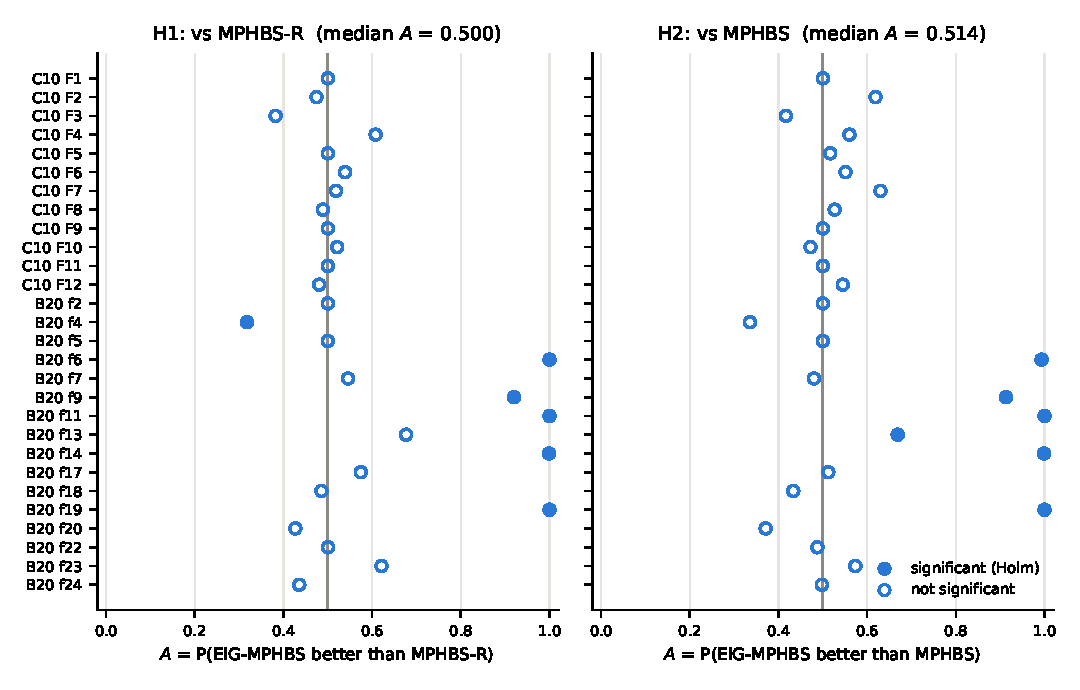
\includegraphics[width=\linewidth]{figures/fig_heldout.pdf}
\caption{Effect size $A$ of EIG-MPHBS on each of the 28 held-out instances against MPHBS-R (H1) and MPHBS (H2);
$A>0.5$ favours EIG-MPHBS. Filled markers: significant per-instance paired test (Holm within benchmark).
C10: CEC2022 $D=10$; B20: BBOB $D=20$.}
\label{fig:heldout}
\end{figure}

\subsection{Rotation dependence}
\label{sec:rotation}
Table~\ref{tab:rotation} compares BBOB functions that differ only by a rotation. On the separable ellipsoid (f2) all
algorithms reach the accuracy floor. On the rotated ellipsoid (f10), MPHBS and MPHBS-R stall at median errors of
\res{f10-MPHBS} and \res{f10-RND}, while EIG-MPHBS reaches \res{f10-EIG50}, a \res{f10-ratio-RND}-fold reduction
relative to MPHBS-R. This is the mechanism the method targets: the exchange in the eigen frame recombines along the
principal axes of the ellipsoid. The gap to CMA-ES and L-SHADE, which solve f10, remains, because Phase 1 of the hybrid
is still coordinate-wise. On Rastrigin, the rotated version (f15) is hard for all three hybrids and the eigen frame does
not help (median \res{f15-EIG50} against \res{f15-RND} for MPHBS-R); on the separable version (f3) EIG-MPHBS is slightly
worse (\res{f3-EIG50} against \res{f3-RND}), as expected when half of the exchanges no longer use the axes along which
the function separates. Multimodal rotated problems need more than a change of frame in the exchange step.

% generated by scripts/eswa_paper_assets.py -- do not edit
\begin{table}[!htbp]
\centering
\caption{Median final error on BBOB function pairs that differ only by a rotation ($D=20$, 30 runs; values at or
below $10^{-8}$ shown as 0).}
\label{tab:rotation}
\small
\begin{tabular}{lcccc}
\toprule
 & \multicolumn{2}{c}{Ellipsoid} & \multicolumn{2}{c}{Rastrigin} \\
\cmidrule(lr){2-3}\cmidrule(lr){4-5}
Algorithm & f2 (separable) & f10 (rotated) & f3 (separable) & f15 (rotated) \\
\midrule
EIG-MPHBS & 0 & 8.47 & 1.99 & 54.2 \\
MPHBS-R & 0 & 89.9 & 0.995 & 58.7 \\
MPHBS & 0 & 121 & 0.995 & 51.2 \\
CMA-ES & 0 & 0 & 8.95 & 2.98 \\
L-SHADE & 0 & 0 & 0 & 4.13 \\
\bottomrule
\end{tabular}
\end{table}


\subsection{Comparison with ten algorithms}
Table~\ref{tab:ranks} gives the mean Friedman ranks of the eleven algorithms and Table~\ref{tab:wtl} the per-instance
significance counts of EIG-MPHBS against each of them; Tables~\ref{tab:med-C10}--\ref{tab:med-FIR} in
\ref{app:tables} give the median errors per instance. The Friedman test rejects equal performance on every benchmark
($p\le\res{friedman-FIR}$).

EIG-MPHBS ranks \res{pos-EIG50} of 11 overall (mean rank \res{rank-EIG50}), behind L-SHADE (\res{rank-L-SHADE}) and
CMA-ES (\res{rank-CMA-ES}) and ahead of MPHBS-R (\res{rank-RND}), MPHBS (\res{rank-MPHBS}) and all classical
metaheuristics. It has the best mean rank on CEC2022 $D=10$ and ranks third on the other three benchmarks.
\begin{itemize}
\item \textbf{Against its own family}, EIG-MPHBS is significantly better than MPHBS on \res{win-MPHBS} instances and
worse on none, and better than MPHBS-R on \res{win-RND} and worse on \res{loss-RND}.
\item \textbf{Against the parent algorithms}, it is significantly better than HBA on \res{win-HBA} of 56 instances and
worse on none, and better than MPA on \res{win-MPA} and worse on \res{loss-MPA}; MPA is the strongest of the classical
algorithms, and many of the ties with it are CEC2022 $D=10$ functions that both solve.
\item \textbf{Against PSO, DE, GWO and WOA}, it is better on \res{win-PSO}, \res{win-DE}, \res{win-GWO} and
\res{win-WOA} instances and worse on \res{loss-PSO}, \res{loss-DE}, \res{loss-GWO} and \res{loss-WOA}. Over the six
classical algorithms it wins \res{common-win} and loses \res{common-loss} of \res{common-n} comparisons.
\item \textbf{Against L-SHADE and CMA-ES}, it is better on \res{win-L-SHADE} and \res{win-CMA-ES} instances and worse on
\res{loss-L-SHADE} and \res{loss-CMA-ES}. On CEC2022 $D=10$ the three are close, but at $D=20$, on BBOB and on FIR the two
references are clearly stronger.
\end{itemize}
GWO and WOA perform poorly on these shifted problems; both are known to be biased towards the centre of the search
space~\citep{kudela2022centre}, which our unit tests confirm on a shifted sphere.

% generated by scripts/eswa_paper_assets.py -- do not edit
\begin{table}[!htbp]
\centering
\caption{Mean Friedman rank of the eleven algorithms (rank of the median final error on each instance, 1 = best;
lowest in bold), per benchmark and over all 56 instances. Last row: Friedman test $p$ per benchmark.}
\label{tab:ranks}
\small
\begin{tabular}{lccccc}
\toprule
Algorithm & C10 & C20 & B20 & FIR & All \\
 & (12) & (12) & (24) & (8) & (56) \\
\midrule
L-SHADE & 3.67 & \textbf{1.71} & \textbf{2.71} & 2.00 & \textbf{2.60} \\
CMA-ES & 4.92 & 2.38 & 2.96 & \textbf{1.00} & 2.97 \\
EIG-MPHBS & \textbf{3.54} & 4.17 & 4.38 & 3.38 & 4.01 \\
MPHBS-R & 3.79 & 4.92 & 5.00 & 4.25 & 4.62 \\
MPHBS & 4.50 & 4.83 & 4.71 & 4.38 & 4.64 \\
MPA & 3.58 & 5.67 & 4.73 & 6.12 & 4.88 \\
DE & 5.83 & 6.33 & 6.19 & 7.88 & 6.38 \\
HBA & 8.12 & 7.92 & 7.54 & 7.00 & 7.67 \\
PSO & 7.71 & 7.75 & 8.17 & 9.88 & 8.22 \\
GWO & 9.50 & 9.33 & 9.04 & 9.50 & 9.27 \\
WOA & 10.83 & 11.00 & 10.58 & 10.62 & 10.73 \\
\midrule
Friedman $p$ & \ensuremath{3.9{\times}10^{-14}} & \ensuremath{1.3{\times}10^{-14}} & \ensuremath{2.8{\times}10^{-26}} & \ensuremath{1.4{\times}10^{-12}} & -- \\
\bottomrule
\end{tabular}
\end{table}

% generated by scripts/eswa_paper_assets.py -- do not edit
\begin{table}[t]
\centering
\caption{EIG-MPHBS against each algorithm: number of instances where it is significantly better / not
significantly different / significantly worse (paired two-sided Wilcoxon signed-rank test over the 30 seed-paired
runs, Holm within each benchmark and comparator, $\alpha=0.05$).}
\label{tab:wtl}
\small
\begin{tabular}{lccccc}
\toprule
vs & C10 (12) & C20 (12) & B20 (24) & FIR (8) & Total (56) \\
\midrule
L-SHADE & 1/9/2 & 0/4/8 & 3/5/16 & 0/0/8 & 4/18/34 \\
CMA-ES & 3/7/2 & 1/5/6 & 4/5/15 & 0/0/8 & 8/17/31 \\
MPHBS-R & 0/12/0 & 3/9/0 & 7/16/1 & 2/6/0 & 12/43/1 \\
MPHBS & 0/12/0 & 2/10/0 & 7/17/0 & 5/3/0 & 14/42/0 \\
MPA & 1/11/0 & 5/5/2 & 10/10/4 & 8/0/0 & 24/26/6 \\
DE & 9/2/1 & 7/3/2 & 13/8/3 & 8/0/0 & 37/13/6 \\
HBA & 10/2/0 & 10/2/0 & 19/5/0 & 8/0/0 & 47/9/0 \\
PSO & 9/3/0 & 9/3/0 & 18/5/1 & 8/0/0 & 44/11/1 \\
GWO & 12/0/0 & 12/0/0 & 20/4/0 & 8/0/0 & 52/4/0 \\
WOA & 12/0/0 & 12/0/0 & 24/0/0 & 8/0/0 & 56/0/0 \\
\bottomrule
\end{tabular}
\end{table}


Fig.~\ref{fig:convergence} shows median convergence curves of seven algorithms on six instances. On BBOB f10, f14 and
f19 and on CEC2022 $D=20$ F\res{conv-C20}, EIG-MPHBS separates from MPHBS and MPHBS-R early and keeps its lead. On f4
the eigen frame slows it down slightly, and on the FIR case shown all three hybrids converge to similar values, with
EIG-MPHBS ahead in mid-run. CMA-ES converges fastest on most instances.

\begin{figure*}[t]
\centering
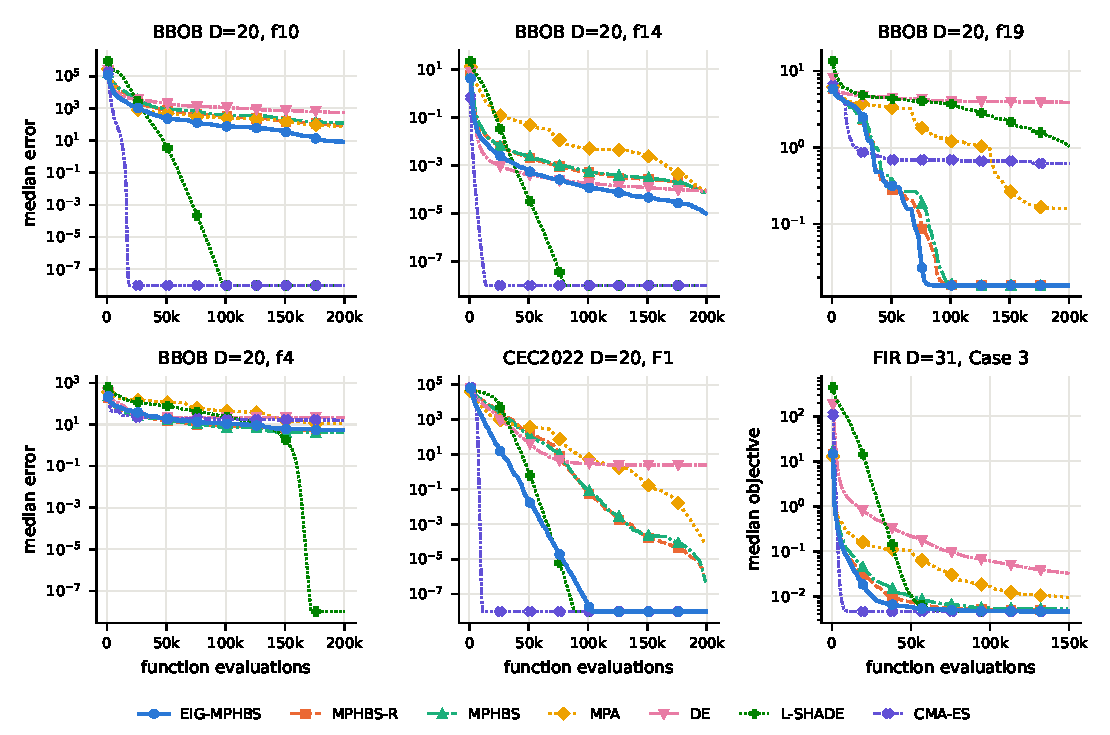
\includegraphics[width=\textwidth]{figures/fig_convergence.pdf}
\caption{Median best-so-far error over 30 runs against function evaluations (FIR: objective value), log scale. The
CEC2022 and FIR instances are those with the strongest per-instance effect of EIG-MPHBS against MPHBS-R; BBOB f4 is
the held-out instance where it is significantly worse.}
\label{fig:convergence}
\end{figure*}

\subsection{Comparison with EA4eig}
EA4eig~\citep{bujok2022ea4eig} combines eigen crossover with four strong algorithms and was among the best entries of
the CEC2022 competition. We compare EIG-MPHBS with the official EA4eig results at the competition budgets (30 runs at
$2\times10^5$ evaluations for $D=10$ and $10^6$ for $D=20$; EIG-MPHBS was rerun at $10^6$ for $D=20$). The comparison is
unpaired and descriptive, because hardware, language and implementation differ. Table~\ref{tab:ea4eig} shows that EA4eig
is significantly better on \res{ea4eig-D10-worse} of 12 functions at $D=10$ and \res{ea4eig-D20-worse} of 12 at $D=20$,
with no significant difference on the rest; EIG-MPHBS is never significantly better. Adding an eigen-frame exchange to
an HBA--MPA hybrid does not close the gap to a cooperative model of state-of-the-art evolutionary algorithms.

% generated by scripts/eswa_paper_assets.py -- do not edit
\begin{table}[t]
\centering
\caption{EIG-MPHBS against the official CEC2022 runs of EA4eig at the competition budgets ($2\times10^5$
evaluations for $D=10$, $10^6$ for $D=20$; 30 runs each). Median final error (at or below $10^{-8}$ shown as 0) and
Vargha--Delaney $A$ ($>0.5$ favours EIG-MPHBS). Superscripts: two-sided Mann--Whitney test, Holm over the 12
functions of each dimension ($^{+}$ EIG-MPHBS better, $^{-}$ worse, $^{\approx}$ no significant difference).
Unpaired and descriptive: hardware and implementation differ.}
\label{tab:ea4eig}
\small
\begin{tabular}{lcccccc}
\toprule
 & \multicolumn{3}{c}{$D=10$} & \multicolumn{3}{c}{$D=20$} \\
\cmidrule(lr){2-4}\cmidrule(lr){5-7}
 & EIG-MPHBS & EA4eig & $A$ & EIG-MPHBS & EA4eig & $A$ \\
\midrule
F1 & 0$^{\approx}$ & 0 & 0.50 & 0$^{\approx}$ & 0 & 0.50 \\
F2 & 0$^{\approx}$ & 0 & 0.46 & 47$^{-}$ & 0 & 0.17 \\
F3 & 2.27e-7$^{-}$ & 0 & 0.13 & 7.77e-8$^{-}$ & 0 & 0.15 \\
F4 & 7.96$^{-}$ & 0.995 & 0.01 & 34.8$^{-}$ & 6.96 & 0.00 \\
F5 & 0$^{\approx}$ & 0 & 0.50 & 14.1$^{-}$ & 0 & 0.00 \\
F6 & 0.155$^{-}$ & 5.41e-3 & 0.04 & 3.28$^{-}$ & 0.106 & 0.01 \\
F7 & 2.36e-6$^{-}$ & 0 & 0.02 & 25.3$^{-}$ & 2.3 & 0.03 \\
F8 & 0.16$^{-}$ & 0.0467 & 0.27 & 20.6$^{-}$ & 20.3 & 0.29 \\
F9 & 229$^{-}$ & 186 & 0.00 & 181$^{-}$ & 165 & 0.00 \\
F10 & 100$^{-}$ & 100 & 0.11 & 100$^{\approx}$ & 100 & 0.34 \\
F11 & 0$^{\approx}$ & 0 & 0.50 & 300$^{-}$ & 300 & 0.16 \\
F12 & 159$^{-}$ & 146 & 0.00 & 240$^{-}$ & 200 & 0.00 \\
\bottomrule
\end{tabular}
\end{table}


\subsection{Computational cost}
\label{sec:cost}
EIG-MPHBS and MPHBS-R used identical evaluation counts on every one of their paired runs, as
Proposition~\ref{prop:cost} states. Table~\ref{tab:cost} reports the run times. The eigen frame adds
\res{overhead-min}--\res{overhead-max}\% to the median run time of MPHBS-R, and EIG-MPHBS is faster than MPHBS, whose
SARSA bookkeeping costs more than the eigendecomposition. The classical algorithms are faster per run because their
iterations are simpler; with expensive objectives, where evaluations dominate, the differences in algorithmic overhead
become negligible.

% generated by scripts/eswa_paper_assets.py -- do not edit
\begin{table}[!htbp]
\centering
\caption{Median wall-clock time per run in seconds (Python 3, NumPy, one core per run, 11 runs in parallel on a
12-core laptop; other jobs shared the machine, so times are indicative). Last row: median paired ratio of the run
times of EIG-MPHBS and MPHBS-R, which use identical evaluation counts.}
\label{tab:cost}
\small
\begin{tabular}{lcccc}
\toprule
Algorithm & C10 & C20 & B20 & FIR \\
\midrule
EIG-MPHBS & 61.3 & 60.9 & 133.2 & 79.8 \\
MPHBS-R & 60.6 & 59.2 & 132.1 & 77.1 \\
MPHBS & 81.1 & 75.9 & 158.3 & 86.9 \\
HBA & 7.1 & 8.4 & 8.4 & 20.5 \\
MPA & 4.5 & 5.7 & 5.7 & 19.2 \\
L-SHADE & 19.4 & 11.6 & 23.4 & 24.9 \\
CMA-ES & 120.8 & 89.1 & 183.2 & 75.6 \\
DE & 17.6 & 18.2 & 18.3 & 28.4 \\
PSO & 4.9 & 6.1 & 5.9 & 19.3 \\
GWO & 5.7 & 7.2 & 7.0 & 18.9 \\
WOA & 5.5 & 6.6 & 6.4 & 17.7 \\
\midrule
EIG-MPHBS / MPHBS-R & 1.055 & 1.033 & 1.032 & 1.032 \\
\bottomrule
\end{tabular}
\end{table}


%% =====================================================================
\section{Discussion}
\label{sec:discussion}

\paragraph{What the eigen frame achieves} The exchange step of HBA--MPA hybrids is where the two populations combine
their information, and it was written for separable problems. Moving it into the eigen frame of the pooled populations
makes it invariant to rotations at no extra evaluation cost, and the results show that this matters: EIG-MPHBS is never
significantly worse than MPHBS on any of 56 instances and is better on \res{win-MPHBS}, with the largest gains on
ill-conditioned rotated functions, on CEC2022 at $D=20$ and on the FIR application. The change is local, a few lines in
the mediator, and should transfer to other hybrids that assemble solutions coordinate by coordinate.

\paragraph{What it does not achieve} The frame helps unimodal or moderately multimodal problems with coupled variables,
where the population covariance reflects the basin; it does not help highly multimodal rotated functions such as f15,
and it costs a little on separable multimodal ones such as f3 and f4, where half of the exchanges no longer follow the
separable axes. Phase 1 remains coordinate-wise, which is why the gap to CMA-ES and L-SHADE on rotated functions
persists. The comparison with EA4eig confirms that this is an improvement of a hybrid within its class, not a new
state of the art.

\paragraph{Practical guidance} For practitioners who use HBA--MPA hybrids, for example because they are already part of
an application pipeline, EIG-MPHBS is a safe replacement for MPHBS: same budget, similar run time, never worse in our
tests and often better. When the choice of algorithm is open, L-SHADE and CMA-ES remain the stronger default on
problems of this size, and the classical metaheuristics PSO, GWO and WOA are clearly weaker than all three hybrids.

\paragraph{Threats to validity} (i) The confirmatory effect is small and sensitive to the handling of tied instances;
the stronger effects come from instances that include the pilot instances. (ii) The value $q=0.5$ was chosen from a
pilot with two values; other values or an adaptive $q$ may perform differently. (iii) The six classical algorithms were
added after the main analysis and are reported descriptively; they use standard settings, not tuned ones. (iv) The
EA4eig comparison is unpaired and across implementations. (v) Run times were measured on a shared laptop. (vi) All
problems have $D\le31$; for larger $D$ the $O(D^3)$ decomposition and the reliability of the covariance estimate from
$2N$ points should be checked.

%% =====================================================================
\section{Conclusion}
\label{sec:conclusion}
We identified the coordinate dependence of the dimension-wise exchange in the HBA--MPA hybrid MPHBS as a structural
weakness on rotated problems and proposed EIG-MPHBS, which performs the exchange in the eigenvector frame of the pooled
populations in half of the iterations. The exchange becomes provably rotation invariant at no extra evaluation cost and
a few percent of extra run time. In \res{runs-total} runs on CEC2022, BBOB and FIR filter design, EIG-MPHBS improved on
MPHBS on \res{win-MPHBS} instances and was never worse, passed a test fixed in advance on 28 held-out instances
(narrowly), and outperformed its parent algorithms and four classical metaheuristics. It ranked third of eleven,
behind L-SHADE and CMA-ES, and remained behind EA4eig at the CEC2022 budgets. Future work includes an adaptive choice of
the frame probability, rotation-invariant versions of the Phase-1 moves, and tests at higher dimension.

\section*{Data and code availability}
Code, the design document (\path{experiments/ESWA_EIGEN_CAMPAIGN.md}), all \res{runs-total} raw runs, the analyses and
the scripts that generate every number, table and figure in this paper are available at
\url{https://github.com/abinaya-g/la-kaie} \pending{campaign commit and release tag}. The EA4eig results are the
official CEC2022 competition files, redistributed with their source in \path{data/external/cec2022_ea4eig/}.

\section*{CRediT authorship contribution statement}
\textbf{Abinaya G:} Conceptualization, Methodology, Software, Validation, Formal analysis, Investigation, Data curation,
Writing -- original draft, Writing -- review \& editing, Visualization.

\section*{Declaration of competing interest}
The author declares that there are no known competing financial interests or personal relationships that could have
appeared to influence the work reported in this paper.

\section*{Funding}
This research did not receive any specific grant from funding agencies in the public, commercial, or not-for-profit
sectors.

\appendix
\section{Median errors per instance}
\label{app:tables}
% generated by scripts/eswa_paper_assets.py -- do not edit
\begin{table}[p]
\centering
\caption{Median final error over 30 runs on CEC2022 $D{=}10$ (FIR: objective value). Errors at or below $10^{-8}$ are shown as 0; lowest median in bold. Superscripts compare with EIG-MPHBS (paired Wilcoxon, Holm within benchmark and comparator): $^{+}$ EIG-MPHBS significantly better, $^{-}$ significantly worse, $^{\approx}$ no significant difference.}
\label{tab:med-C10}
\resizebox{\textwidth}{!}{%
\begin{tabular}{lrrrrrrrrrrr}
\toprule
 & EIG-MPHBS & MPHBS-R & MPHBS & HBA & MPA & L-SHADE & CMA-ES & DE & PSO & GWO & WOA \\
\midrule
F1 & \textbf{0} & \textbf{0}$^{\approx}$ & \textbf{0}$^{\approx}$ & \textbf{0}$^{\approx}$ & \textbf{0}$^{\approx}$ & \textbf{0}$^{\approx}$ & \textbf{0}$^{\approx}$ & 0.0805$^{+}$ & \textbf{0}$^{\approx}$ & 137$^{+}$ & 8.29e+03$^{+}$ \\
F2 & \textbf{0} & \textbf{0}$^{\approx}$ & 3.99$^{\approx}$ & 4.09$^{+}$ & \textbf{0}$^{\approx}$ & 3.99$^{\approx}$ & 3.99$^{\approx}$ & 8.92$^{+}$ & 8.92$^{+}$ & 10.4$^{+}$ & 76$^{+}$ \\
F3 & 2.27e-7 & 2.46e-8$^{\approx}$ & 9.39e-8$^{\approx}$ & 5.75e-5$^{+}$ & 2.98e-5$^{+}$ & \textbf{0}$^{-}$ & \textbf{0}$^{-}$ & \textbf{0}$^{-}$ & \textbf{0}$^{\approx}$ & 0.131$^{+}$ & 34.8$^{+}$ \\
F4 & 7.96 & 8.95$^{\approx}$ & 8.95$^{\approx}$ & 15.9$^{+}$ & 6.96$^{\approx}$ & 2.98$^{-}$ & \textbf{0.995}$^{-}$ & 9.79$^{+}$ & 10.4$^{\approx}$ & 14.1$^{+}$ & 39$^{+}$ \\
F5 & \textbf{0} & \textbf{0}$^{\approx}$ & \textbf{0}$^{\approx}$ & 0.544$^{+}$ & \textbf{0}$^{\approx}$ & \textbf{0}$^{\approx}$ & \textbf{0}$^{\approx}$ & \textbf{0}$^{+}$ & \textbf{0}$^{+}$ & 1.36$^{+}$ & 402$^{+}$ \\
F6 & 0.155 & 0.178$^{\approx}$ & 0.169$^{\approx}$ & 1.42e+03$^{+}$ & \textbf{0.138}$^{\approx}$ & 0.311$^{+}$ & 0.49$^{+}$ & 2.56$^{+}$ & 3.35e+03$^{+}$ & 2.9e+03$^{+}$ & 2.25e+03$^{+}$ \\
F7 & 2.36e-6 & 4.83e-6$^{\approx}$ & 0.995$^{\approx}$ & 21$^{+}$ & 0.995$^{\approx}$ & \textbf{1.63e-6}$^{\approx}$ & 1.62$^{\approx}$ & 0.667$^{\approx}$ & 20.6$^{+}$ & 23.3$^{+}$ & 96.2$^{+}$ \\
F8 & 0.16 & 0.18$^{\approx}$ & 0.232$^{\approx}$ & 21$^{+}$ & \textbf{0.138}$^{\approx}$ & 0.669$^{\approx}$ & 17.3$^{+}$ & 0.763$^{+}$ & 20.7$^{+}$ & 24.5$^{+}$ & 32.4$^{+}$ \\
F9 & \textbf{229} & \textbf{229}$^{\approx}$ & \textbf{229}$^{\approx}$ & 230$^{+}$ & \textbf{229}$^{\approx}$ & \textbf{229}$^{\approx}$ & \textbf{229}$^{\approx}$ & \textbf{229}$^{\approx}$ & 230$^{+}$ & 231$^{+}$ & 388$^{+}$ \\
F10 & 100 & 100$^{\approx}$ & 100$^{\approx}$ & 210$^{+}$ & 100$^{\approx}$ & \textbf{100}$^{\approx}$ & 100$^{\approx}$ & 100$^{+}$ & 210$^{+}$ & 207$^{+}$ & 253$^{+}$ \\
F11 & \textbf{0} & \textbf{0}$^{\approx}$ & \textbf{0}$^{\approx}$ & \textbf{0}$^{\approx}$ & \textbf{0}$^{\approx}$ & \textbf{0}$^{\approx}$ & \textbf{0}$^{\approx}$ & \textbf{0}$^{+}$ & 178$^{+}$ & 130$^{+}$ & 279$^{+}$ \\
F12 & 159 & \textbf{159}$^{\approx}$ & 160$^{\approx}$ & 183$^{+}$ & 160$^{\approx}$ & 161$^{\approx}$ & 163$^{+}$ & 164$^{+}$ & 171$^{+}$ & 164$^{+}$ & 233$^{+}$ \\
\bottomrule
\end{tabular}}
\end{table}

% generated by scripts/eswa_paper_assets.py -- do not edit
\begin{table*}[p]
\centering
\caption{Median final error over 30 runs on CEC2022 $D{=}20$ (FIR: objective value). Errors at or below $10^{-8}$ are shown as 0; lowest median in bold. Superscripts compare with EIG-MPHBS (paired Wilcoxon, Holm within benchmark and comparator): $^{+}$ EIG-MPHBS significantly better, $^{-}$ significantly worse, $^{\approx}$ no significant difference.}
\label{tab:med-C20}
\resizebox{\textwidth}{!}{%
\begin{tabular}{lrrrrrrrrrrr}
\toprule
 & EIG-MPHBS & MPHBS-R & MPHBS & HBA & MPA & L-SHADE & CMA-ES & DE & PSO & GWO & WOA \\
\midrule
F1 & \textbf{0} & 2.18e-7$^{+}$ & 2.82e-7$^{+}$ & 2.69e-8$^{+}$ & 5.13e-5$^{+}$ & \textbf{0}$^{\approx}$ & \textbf{0}$^{\approx}$ & 2.51$^{+}$ & 2.77e-8$^{+}$ & 3.97e+03$^{+}$ & 3.30e4$^{+}$ \\
F2 & 44.9 & 49.1$^{+}$ & 44.9$^{\approx}$ & 49.1$^{\approx}$ & 44.9$^{\approx}$ & 49.1$^{\approx}$ & \textbf{44.9}$^{\approx}$ & 49.1$^{+}$ & 54.4$^{+}$ & 93$^{+}$ & 653$^{+}$ \\
F3 & 1.72e-5 & 5.03e-6$^{\approx}$ & 6.93e-6$^{\approx}$ & 1.09$^{+}$ & 4.68e-3$^{+}$ & \textbf{0}$^{-}$ & \textbf{0}$^{-}$ & 2.33e-5$^{\approx}$ & 0.556$^{+}$ & 2.29$^{+}$ & 71.7$^{+}$ \\
F4 & 35.3 & 36.8$^{\approx}$ & 30.3$^{\approx}$ & 50.7$^{+}$ & 38.8$^{\approx}$ & 5.97$^{-}$ & \textbf{3.98}$^{-}$ & 19.5$^{-}$ & 38$^{\approx}$ & 44.3$^{+}$ & 148$^{+}$ \\
F5 & 16.3 & 15.4$^{\approx}$ & 26.5$^{\approx}$ & 161$^{+}$ & 14.9$^{\approx}$ & \textbf{0}$^{-}$ & \textbf{0}$^{-}$ & 0.499$^{-}$ & 8.15$^{\approx}$ & 158$^{+}$ & 2.32e+03$^{+}$ \\
F6 & 12.2 & 16.8$^{\approx}$ & 24$^{\approx}$ & 2.46e+03$^{+}$ & 10.6$^{\approx}$ & \textbf{0.489}$^{-}$ & 52.5$^{+}$ & 3.21e+03$^{+}$ & 2.45e+03$^{+}$ & 2.08e4$^{+}$ & 7.11e7$^{+}$ \\
F7 & 31.1 & 29.8$^{\approx}$ & 27.4$^{\approx}$ & 69.1$^{+}$ & 24.9$^{-}$ & \textbf{20.3}$^{-}$ & 21.6$^{-}$ & 24.2$^{\approx}$ & 29.2$^{\approx}$ & 51.8$^{+}$ & 200$^{+}$ \\
F8 & 21 & 21$^{\approx}$ & 21.2$^{\approx}$ & 24.9$^{+}$ & 21.1$^{\approx}$ & 20.9$^{\approx}$ & \textbf{20.8}$^{\approx}$ & 22.2$^{+}$ & 41.3$^{+}$ & 28.3$^{+}$ & 58.2$^{+}$ \\
F9 & 181 & 181$^{+}$ & 181$^{+}$ & 181$^{+}$ & 181$^{+}$ & \textbf{181}$^{-}$ & \textbf{181}$^{-}$ & 181$^{+}$ & 218$^{+}$ & 208$^{+}$ & 443$^{+}$ \\
F10 & 100 & 100$^{\approx}$ & 100$^{\approx}$ & 839$^{+}$ & 101$^{+}$ & \textbf{100}$^{\approx}$ & 100$^{\approx}$ & 101$^{+}$ & 292$^{+}$ & 912$^{+}$ & 3.26e+03$^{+}$ \\
F11 & 300 & 300$^{\approx}$ & 300$^{\approx}$ & 300$^{\approx}$ & 400$^{+}$ & \textbf{300}$^{-}$ & 300$^{\approx}$ & 303$^{\approx}$ & 966$^{+}$ & 748$^{+}$ & 2.9e+03$^{+}$ \\
F12 & 243 & 239$^{\approx}$ & 241$^{\approx}$ & 357$^{+}$ & 241$^{-}$ & \textbf{234}$^{-}$ & 236$^{-}$ & 246$^{+}$ & 285$^{+}$ & 261$^{+}$ & 504$^{+}$ \\
\bottomrule
\end{tabular}}
\end{table*}

% generated by scripts/eswa_paper_assets.py -- do not edit
\begin{table}[p]
\centering
\caption{Median final error over 30 runs on BBOB $D{=}20$ (FIR: objective value). Errors at or below $10^{-8}$ are shown as 0; lowest median in bold. Superscripts compare with EIG-MPHBS (paired Wilcoxon, Holm within benchmark and comparator): $^{+}$ EIG-MPHBS significantly better, $^{-}$ significantly worse, $^{\approx}$ no significant difference.}
\label{tab:med-B20}
\resizebox{\textwidth}{!}{%
\begin{tabular}{lrrrrrrrrrrr}
\toprule
 & EIG-MPHBS & MPHBS-R & MPHBS & HBA & MPA & L-SHADE & CMA-ES & DE & PSO & GWO & WOA \\
\midrule
f1 & \textbf{0} & \textbf{0}$^{\approx}$ & \textbf{0}$^{\approx}$ & \textbf{0}$^{\approx}$ & \textbf{0}$^{\approx}$ & \textbf{0}$^{\approx}$ & \textbf{0}$^{\approx}$ & \textbf{0}$^{\approx}$ & 1.19$^{+}$ & 0.536$^{+}$ & 15.3$^{+}$ \\
f2 & \textbf{0} & \textbf{0}$^{\approx}$ & \textbf{0}$^{\approx}$ & \textbf{0}$^{\approx}$ & 3.77e-4$^{+}$ & \textbf{0}$^{\approx}$ & \textbf{0}$^{\approx}$ & 0.295$^{+}$ & 3.46e+03$^{+}$ & 1.50e4$^{+}$ & 1.78e5$^{+}$ \\
f3 & 1.99 & 0.995$^{\approx}$ & 0.995$^{\approx}$ & 35.3$^{+}$ & 5.47$^{+}$ & \textbf{0}$^{-}$ & 8.95$^{+}$ & 13.1$^{+}$ & 19$^{+}$ & 45.6$^{+}$ & 337$^{+}$ \\
f4 & 5.47 & 4.97$^{-}$ & 3.98$^{\approx}$ & 45.3$^{+}$ & 10.9$^{+}$ & \textbf{0}$^{-}$ & 15.9$^{+}$ & 21.9$^{+}$ & 17.9$^{+}$ & 66.2$^{+}$ & 357$^{+}$ \\
f5 & \textbf{0} & \textbf{0}$^{\approx}$ & \textbf{0}$^{\approx}$ & 92.1$^{+}$ & \textbf{0}$^{\approx}$ & \textbf{0}$^{\approx}$ & \textbf{0}$^{\approx}$ & \textbf{0}$^{\approx}$ & 30.8$^{+}$ & 10.8$^{+}$ & 106$^{+}$ \\
f6 & 3.26e-8 & 1.78e-6$^{+}$ & 3.37e-6$^{+}$ & 5.41e-4$^{+}$ & 1.06e-4$^{+}$ & \textbf{0}$^{-}$ & \textbf{0}$^{-}$ & \textbf{0}$^{\approx}$ & 114$^{+}$ & 40.8$^{+}$ & 1.19e+03$^{+}$ \\
f7 & 4.31 & 3.59$^{\approx}$ & 2.62$^{\approx}$ & 7.55$^{+}$ & 2.05$^{\approx}$ & \textbf{0}$^{-}$ & \textbf{0}$^{-}$ & 2.62$^{\approx}$ & 13.1$^{+}$ & 14.5$^{+}$ & 183$^{+}$ \\
f8 & 3.64e-7 & 4.22e-4$^{+}$ & 1.84e-3$^{+}$ & 3.31$^{+}$ & 10.7$^{+}$ & \textbf{0}$^{-}$ & \textbf{0}$^{-}$ & 17.2$^{+}$ & 12.8$^{+}$ & 90.7$^{+}$ & 2.82e+03$^{+}$ \\
f9 & 7.03e-3 & 0.798$^{+}$ & 1.48$^{+}$ & 6.41$^{+}$ & 4.57$^{+}$ & \textbf{0}$^{-}$ & \textbf{0}$^{-}$ & 17.7$^{+}$ & 16.9$^{+}$ & 22$^{+}$ & 107$^{+}$ \\
f10 & 8.47 & 89.9$^{+}$ & 121$^{+}$ & 829$^{+}$ & 77.3$^{+}$ & \textbf{0}$^{-}$ & \textbf{0}$^{-}$ & 550$^{+}$ & 7.09e+03$^{+}$ & 1.15e4$^{+}$ & 2.28e5$^{+}$ \\
f11 & \textbf{0} & 3.36e-3$^{+}$ & 8.62e-3$^{+}$ & 1.09$^{+}$ & 4.60e-4$^{+}$ & \textbf{0}$^{\approx}$ & \textbf{0}$^{\approx}$ & 2.65$^{+}$ & 1.65$^{+}$ & 40.4$^{+}$ & 111$^{+}$ \\
f12 & 4.65 & 3.47$^{\approx}$ & 4.35$^{\approx}$ & 3.45$^{\approx}$ & 5.16$^{\approx}$ & \textbf{0}$^{-}$ & \textbf{0}$^{-}$ & 1.96$^{\approx}$ & 7.93e4$^{+}$ & 2.46e5$^{+}$ & 2.85e7$^{+}$ \\
f13 & 0.774 & 2.82$^{\approx}$ & 2.86$^{\approx}$ & 3$^{+}$ & 1.13$^{\approx}$ & \textbf{0}$^{-}$ & \textbf{0}$^{-}$ & 2.04$^{+}$ & 200$^{+}$ & 179$^{+}$ & 858$^{+}$ \\
f14 & 9.73e-6 & 7.96e-5$^{+}$ & 7.21e-5$^{+}$ & 7.79e-5$^{+}$ & 9.53e-5$^{+}$ & \textbf{0}$^{-}$ & \textbf{0}$^{-}$ & 8.40e-5$^{+}$ & 1.58$^{+}$ & 0.26$^{+}$ & 8.69$^{+}$ \\
f15 & 54.2 & 58.7$^{\approx}$ & 51.2$^{\approx}$ & 70.1$^{+}$ & 37.3$^{-}$ & 4.13$^{-}$ & \textbf{2.98}$^{-}$ & 19$^{-}$ & 57.1$^{\approx}$ & 63.9$^{+}$ & 359$^{+}$ \\
f16 & 1.84 & 1.99$^{\approx}$ & 1.92$^{\approx}$ & 6.02$^{+}$ & 1.39$^{\approx}$ & 3.83$^{+}$ & \textbf{0.0403}$^{-}$ & 9.82$^{+}$ & 3.21$^{+}$ & 1.28$^{\approx}$ & 15.8$^{+}$ \\
f17 & 0.488 & 0.592$^{\approx}$ & 0.448$^{\approx}$ & 1.38$^{+}$ & 0.271$^{\approx}$ & \textbf{0}$^{-}$ & \textbf{0}$^{-}$ & 0.0333$^{-}$ & 0.753$^{\approx}$ & 0.918$^{\approx}$ & 7.25$^{+}$ \\
f18 & 1.04 & 1.15$^{\approx}$ & 0.86$^{\approx}$ & 4.83$^{+}$ & 0.997$^{\approx}$ & 4.66e-8$^{-}$ & \textbf{0}$^{-}$ & 0.241$^{-}$ & 1.62$^{\approx}$ & 2.31$^{+}$ & 26.9$^{+}$ \\
f19 & \textbf{0.0157} & 0.0157$^{+}$ & 0.0157$^{+}$ & 0.023$^{+}$ & 0.159$^{+}$ & 1.04$^{+}$ & 0.616$^{+}$ & 3.9$^{+}$ & 3.65$^{+}$ & 3.32$^{+}$ & 0.247$^{+}$ \\
f20 & 1 & 0.987$^{\approx}$ & 0.972$^{\approx}$ & 1.37$^{+}$ & 1.08$^{\approx}$ & \textbf{0.221}$^{-}$ & 1.15$^{\approx}$ & 0.898$^{\approx}$ & 0.75$^{-}$ & 1.52$^{+}$ & 5.68$^{+}$ \\
f21 & 2.04 & 1.92$^{\approx}$ & 1.8$^{\approx}$ & 2.82$^{\approx}$ & \textbf{0.346}$^{-}$ & 1.8$^{-}$ & 0.93$^{-}$ & 2.04$^{\approx}$ & 2.52$^{\approx}$ & 5.27$^{\approx}$ & 27.5$^{+}$ \\
f22 & 8.74 & 8.74$^{\approx}$ & 8.74$^{\approx}$ & 8.74$^{\approx}$ & \textbf{1.32}$^{-}$ & 7.27$^{\approx}$ & 1.91$^{-}$ & 2.59$^{\approx}$ & 8.65$^{\approx}$ & 7.4$^{\approx}$ & 36.2$^{+}$ \\
f23 & \textbf{0.0735} & 0.0948$^{\approx}$ & 0.0802$^{\approx}$ & 1.72$^{+}$ & 0.106$^{\approx}$ & 0.569$^{+}$ & 1.61$^{+}$ & 1.9$^{+}$ & 1.51$^{+}$ & 1.82$^{+}$ & 1.46$^{+}$ \\
f24 & 62.5 & 58$^{\approx}$ & 62.1$^{\approx}$ & 89.9$^{+}$ & 36.8$^{-}$ & 32.6$^{-}$ & \textbf{23.5}$^{-}$ & 102$^{+}$ & 109$^{+}$ & 137$^{+}$ & 182$^{+}$ \\
\bottomrule
\end{tabular}}
\end{table}

% generated by scripts/eswa_paper_assets.py -- do not edit
\begin{table}[p]
\centering
\caption{Median final error over 30 runs on FIR $D{=}31$ (FIR: objective value). Errors at or below $10^{-8}$ are shown as 0; lowest median in bold. Superscripts compare with EIG-MPHBS (paired Wilcoxon, Holm within benchmark and comparator): $^{+}$ EIG-MPHBS significantly better, $^{-}$ significantly worse, $^{\approx}$ no significant difference.}
\label{tab:med-FIR}
\resizebox{\textwidth}{!}{%
\begin{tabular}{lrrrrrrrrrrr}
\toprule
 & EIG-MPHBS & MPHBS-R & MPHBS & HBA & MPA & L-SHADE & CMA-ES & DE & PSO & GWO & WOA \\
\midrule
Case 1 & 4.64e-3 & 4.98e-3$^{+}$ & 5.01e-3$^{+}$ & 0.0113$^{+}$ & 9.09e-3$^{+}$ & 4.56e-3$^{-}$ & \textbf{4.56e-3}$^{-}$ & 0.0306$^{+}$ & 0.0982$^{+}$ & 0.165$^{+}$ & 0.62$^{+}$ \\
Case 2 & 0.0207 & 0.0209$^{\approx}$ & 0.0209$^{\approx}$ & 0.0351$^{+}$ & 0.0302$^{+}$ & 0.0188$^{-}$ & \textbf{0.017}$^{-}$ & 0.0662$^{+}$ & 0.144$^{+}$ & 0.181$^{+}$ & 0.705$^{+}$ \\
Case 3 & 4.61e-3 & 4.90e-3$^{+}$ & 5.19e-3$^{+}$ & 0.0118$^{+}$ & 9.29e-3$^{+}$ & 4.56e-3$^{-}$ & \textbf{4.56e-3}$^{-}$ & 0.0321$^{+}$ & 0.0685$^{+}$ & 0.185$^{+}$ & 0.925$^{+}$ \\
Case 4 & 0.0199 & 0.0213$^{\approx}$ & 0.0213$^{+}$ & 0.0344$^{+}$ & 0.0279$^{+}$ & 0.017$^{-}$ & \textbf{0.017}$^{-}$ & 0.0616$^{+}$ & 0.141$^{+}$ & 0.166$^{+}$ & 0.96$^{+}$ \\
Case 5 & 1.40e-3 & 1.42e-3$^{\approx}$ & 1.73e-3$^{+}$ & 5.62e-3$^{+}$ & 4.31e-3$^{+}$ & 9.68e-4$^{-}$ & \textbf{8.88e-4}$^{-}$ & 0.0671$^{+}$ & 1.87$^{+}$ & 0.0837$^{+}$ & 0.943$^{+}$ \\
Case 6 & 6.17e-3 & 6.21e-3$^{\approx}$ & 5.87e-3$^{\approx}$ & 9.94e-3$^{+}$ & 9.74e-3$^{+}$ & 4.70e-3$^{-}$ & \textbf{4.70e-3}$^{-}$ & 0.069$^{+}$ & 0.226$^{+}$ & 0.0889$^{+}$ & 0.948$^{+}$ \\
Case 7 & 1.37e-3 & 1.36e-3$^{\approx}$ & 1.30e-3$^{\approx}$ & 5.21e-3$^{+}$ & 7.21e-3$^{+}$ & 8.15e-4$^{-}$ & \textbf{6.12e-4}$^{-}$ & 0.0358$^{+}$ & 2.69$^{+}$ & 0.0818$^{+}$ & 0.533$^{+}$ \\
Case 8 & 3.23e-3 & 3.81e-3$^{\approx}$ & 3.89e-3$^{+}$ & 0.0119$^{+}$ & 8.38e-3$^{+}$ & 1.81e-3$^{-}$ & \textbf{1.35e-3}$^{-}$ & 0.0117$^{+}$ & 2.58$^{+}$ & 0.096$^{+}$ & 0.48$^{+}$ \\
\bottomrule
\end{tabular}}
\end{table}


\FloatBarrier
\bibliographystyle{elsarticle-harv}
\bibliography{refs}

\end{document}
